
\section{Multiclass Kernel SVMs}


\subsection{Multiclass SVM strategies}

\subsubsection{spoc-svc}

See \cite{spoc-svc} for details.


\subsubsection{kbb-svc}

See \cite{kbb-svc} for details.


\subsubsection{one-vs-all approach}

The idea is to train one model for each class, that predicts whether a sample belongs to the class or not.
We use KSVM for regression in order to avoid conflicts, which would arise when we would only use binary classification
(i.e. multiple models or no model could predict ``yes'' for the same sample).
Then we can finally predict the class where the model was the most confident (i.e. the regression output is the highest).

\subsubsection{tree-based approach}



\subsection{Parameter optimization}

\subsubsection{spoc-svc}

\subsubsection{kbb-svc}

\subsubsection{one-vs-all approach}

We decided to use the RBF-kernel and the same C-parameter for all of the 10 models,
in order to reduce the parameter searchspace.\\
The following plot shows the validation error for different C-parameters.

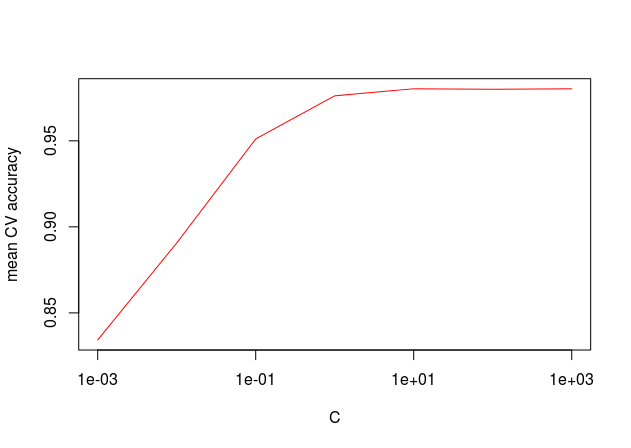
\includegraphics[width=0.8\textwidth]{../plots/one_vs_all_zip}

\subsubsection{tree-based approach}


\subsection{Results}